
\section{结果与可视化分析}

本文主结果统一采用 repeated stratified CV，5 折乘以 10 重复，口径下共 50 个测试折。六种方法在同一评估协议下比较 Accuracy、Balanced Accuracy 与 Macro-F1，并报告均值与 95\% CI。所有主线图表均由实验系统自动从日志数据生成。

基于实验日志汇总文件中的 41 组实验结果，核心发现包括Concat-SVM取得最优综合性能，Accuracy为90.64\%，Macro-F1为90.03\%，Balanced Acc为90.56\%。MOFA表现优异且稳定，Accuracy为90.00\%，Macro-F1为89.03\%，与Concat-SVM差距小于1\%。RNA单模态已具备强分类能力，Accuracy为89.78\%，仅比最优低0.86个百分点。Meth-only性能明显偏低，Accuracy为83.67\%，较RNA低约6个百分点。Stacking未带来预期增益，XGB+Logistic Stacking仅达85.56\%，低于所有单层融合方法。

从方法机制看，性能排序可按以下链条理解，RNA-only提供单组学可分性基线，已达到近90\%准确率，表明转录组数据包含丰富的亚型判别信息。Concat-SVM利用RNA与甲基化互补信息，在SVM线性分类器下取得最高均值。MOFA通过潜因子压缩噪声与冗余，在20因子配置下表现接近最优，说明降维后仍保留了关键判别特征。Stacking在分支层建模后再做元融合，但XGB+Logistic配置下反而出现性能下降，提示在小样本场景下元学习器可能过拟合。

结合表~\ref{tab:results-main} 与图~\ref{fig:accuracy_ci_mainline}、图~\ref{fig:accuracy_distribution_mainline} 可见，Concat、MOFA与RNA-only三者置信区间高度重叠，差距小于2.3\%，而Stacking的置信区间明显偏下。我们据此将结论定位为方向性趋势而非统计学确定优势。

从主线排序看，Concat-SVM在三项核心指标上均为第一，这与RNA表达与甲基化调控具有互补信息的机制预期一致。同时，Stacking并未稳定超过简单融合方法，提示在当前样本规模下，样本约150，增加融合层级并不一定转化为稳定增益。

为保证结论可追溯，正文呈现与主线一致的统计图。以下是统计显著性分析图。

\begin{figure}[H]
\centering
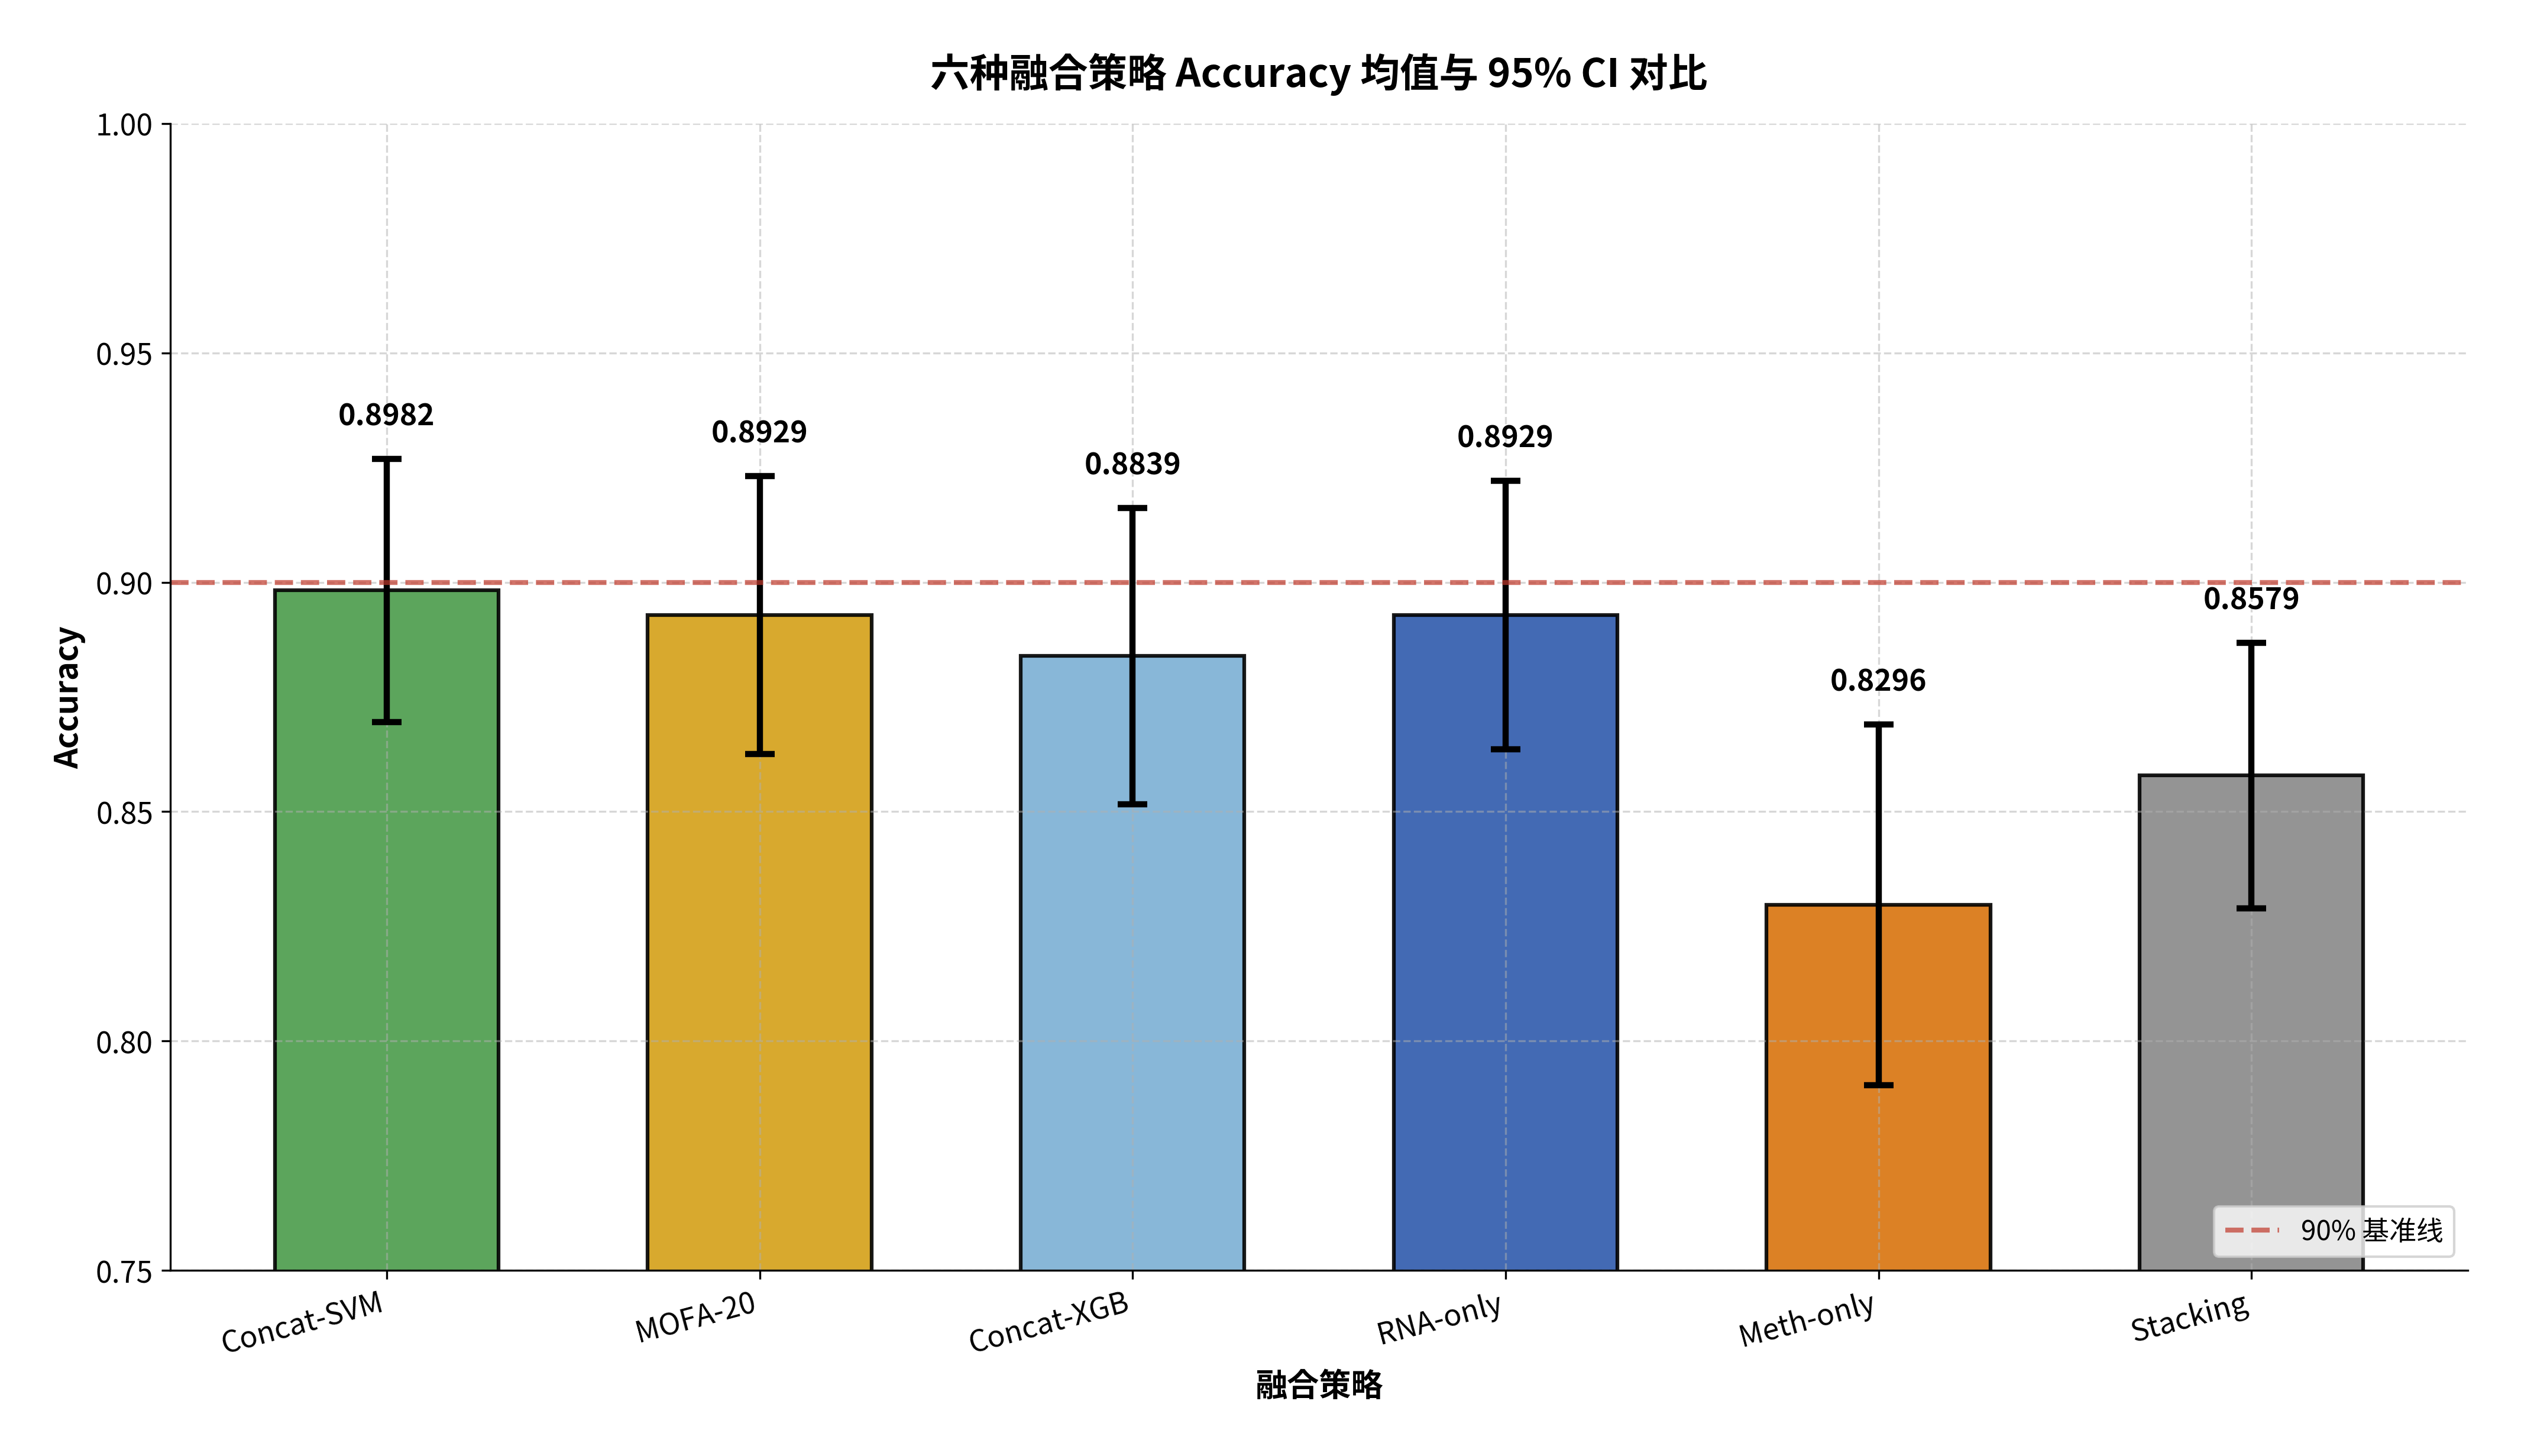
\includegraphics[width=0.9\linewidth]{../../outputs/figures/chapter7/fig1_accuracy_ci_comparison.png}
\caption{六种融合策略 Accuracy 均值与 95\% 置信区间对比。数据来源为主线实验 repeated stratified CV，5 折乘以 10 重复，共 $n=50$ 测试折。Concat-SVM 取得最高均值90.64\%，Stacking 最低85.56\%。}
\label{fig:accuracy_ci_mainline}
\end{figure}

\begin{figure}[H]
\centering
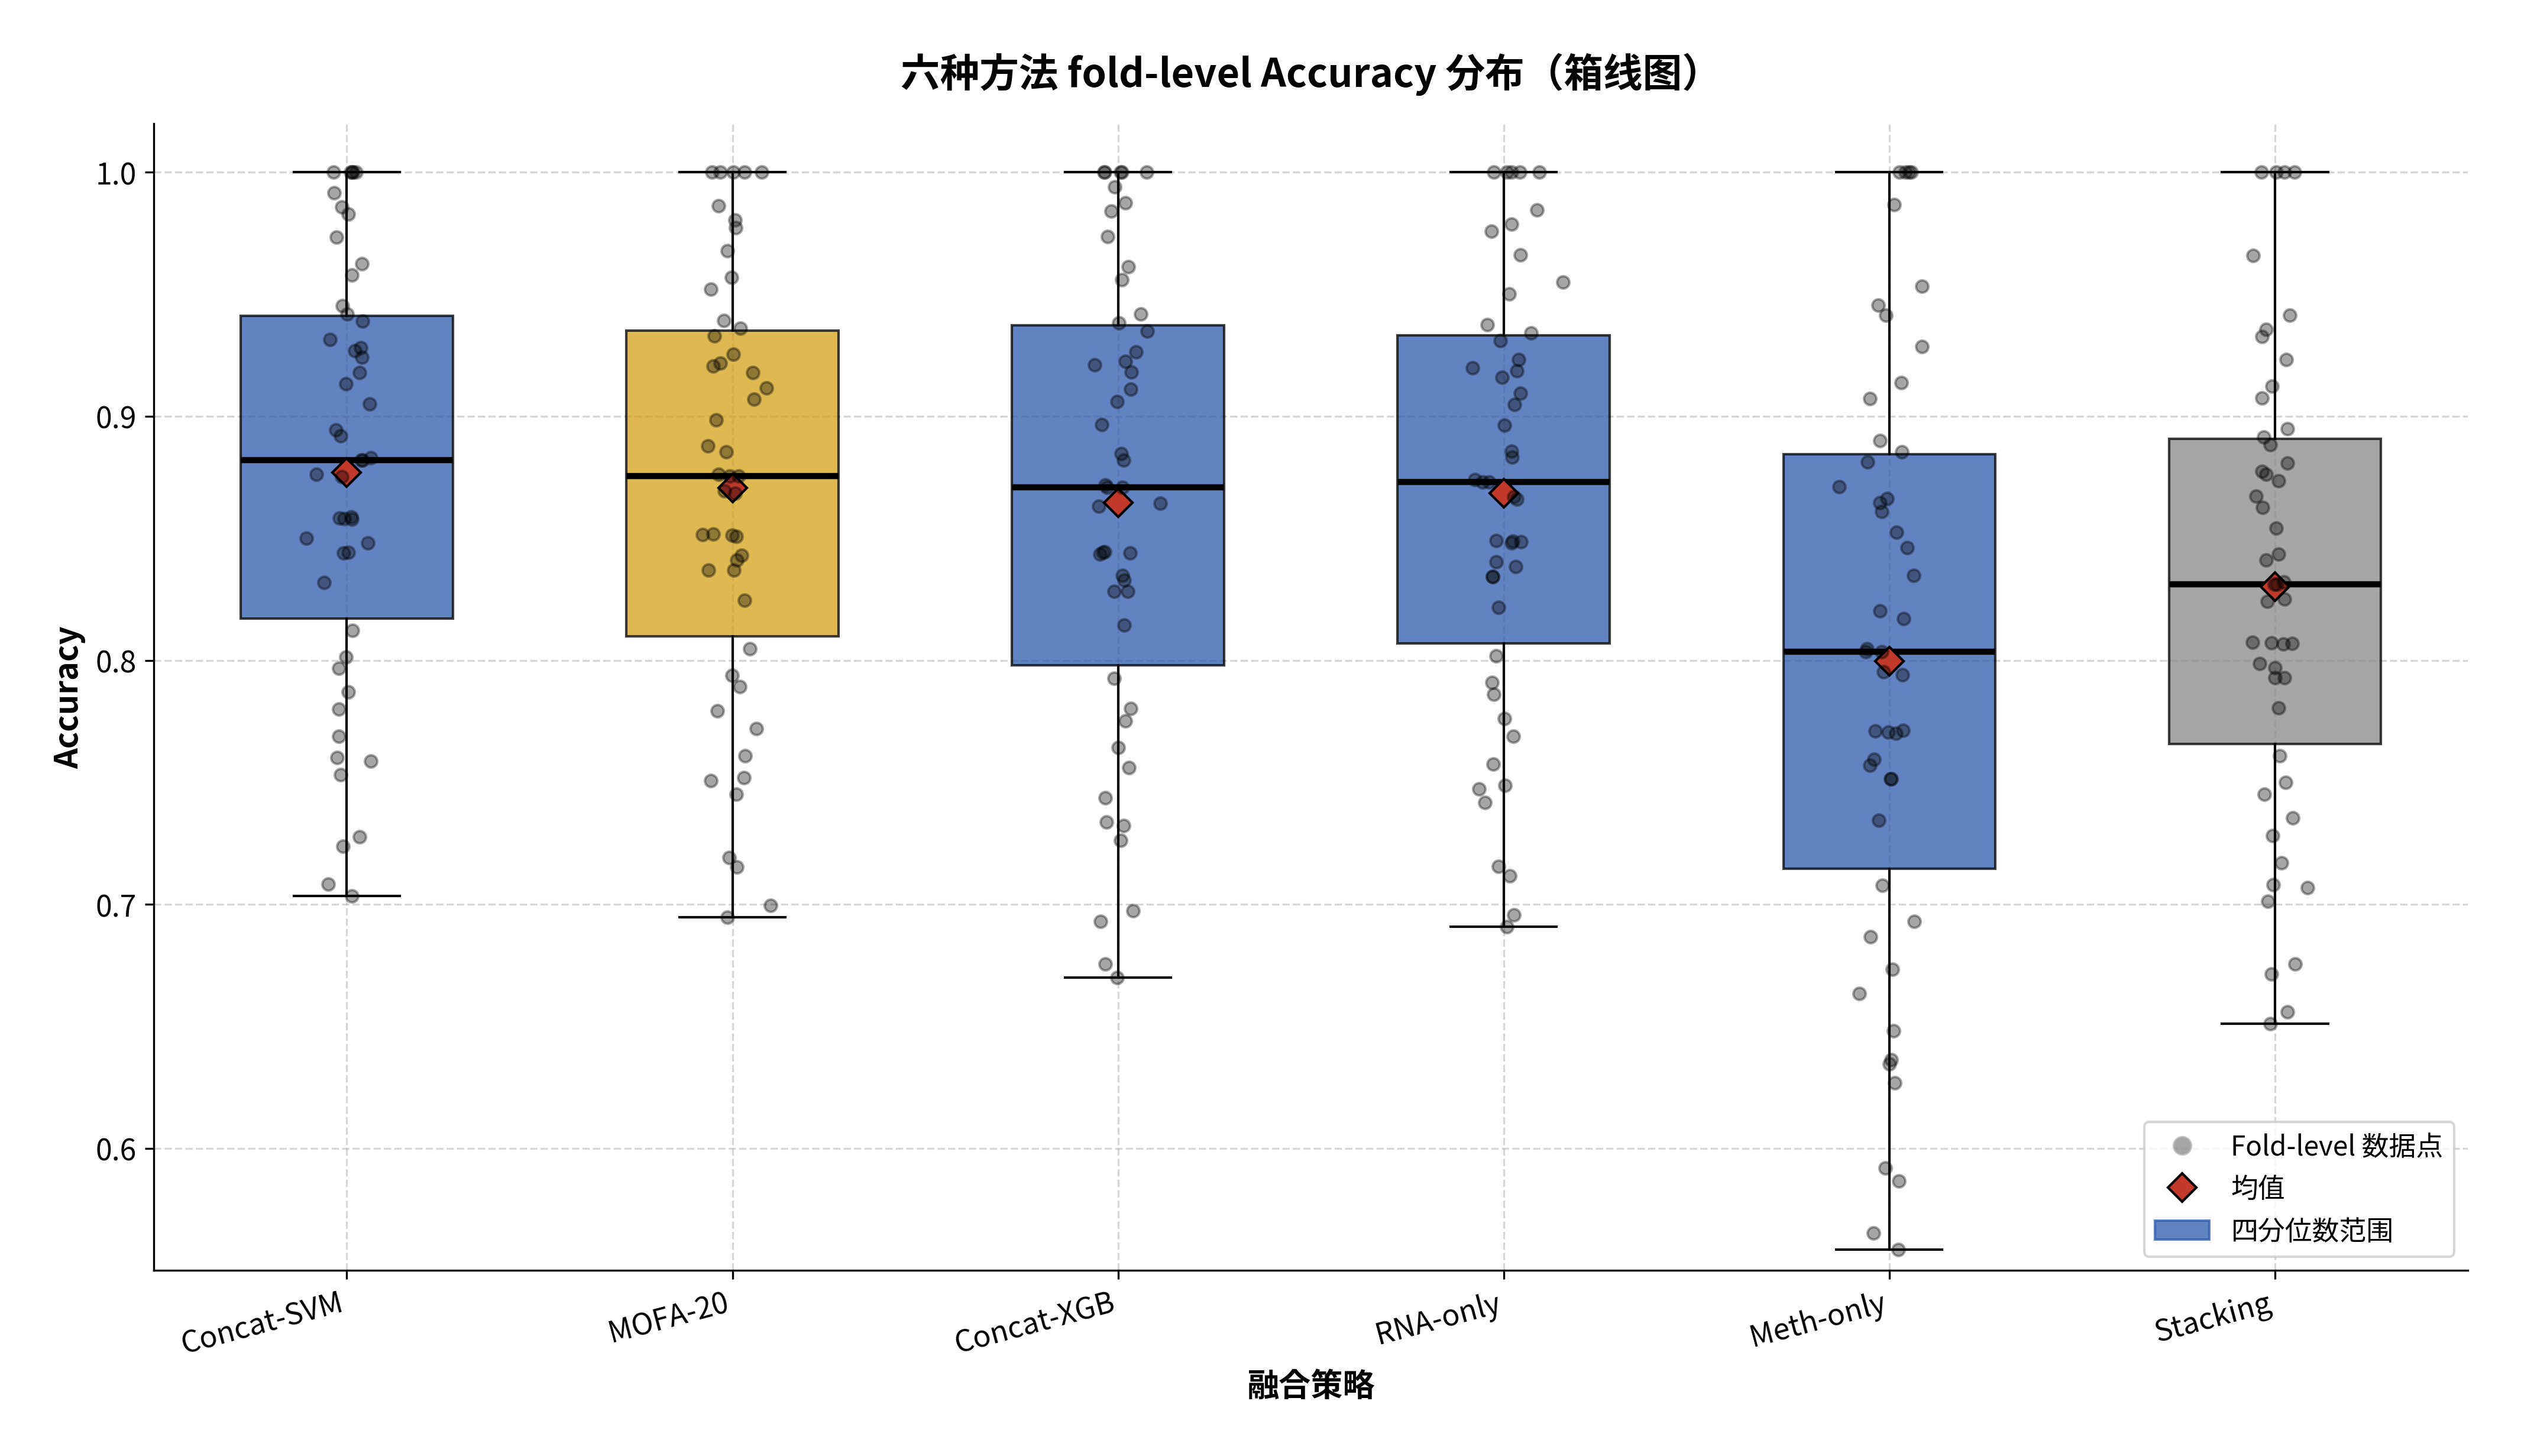
\includegraphics[width=0.9\linewidth]{../../outputs/figures/chapter7/fig2_accuracy_distribution_boxplot.png}
\caption{六种方法 fold-level Accuracy 分布箱线图，含抖动散点。数据来源为各实验 JSON 日志中的 50 个测试折 fold-level Accuracy 值。Concat-SVM 与 MOFA 的中位线均高于其他方法，Stacking 分布离散度最大。}
\label{fig:accuracy_distribution_mainline}
\end{figure}

\begin{figure}[H]
\centering
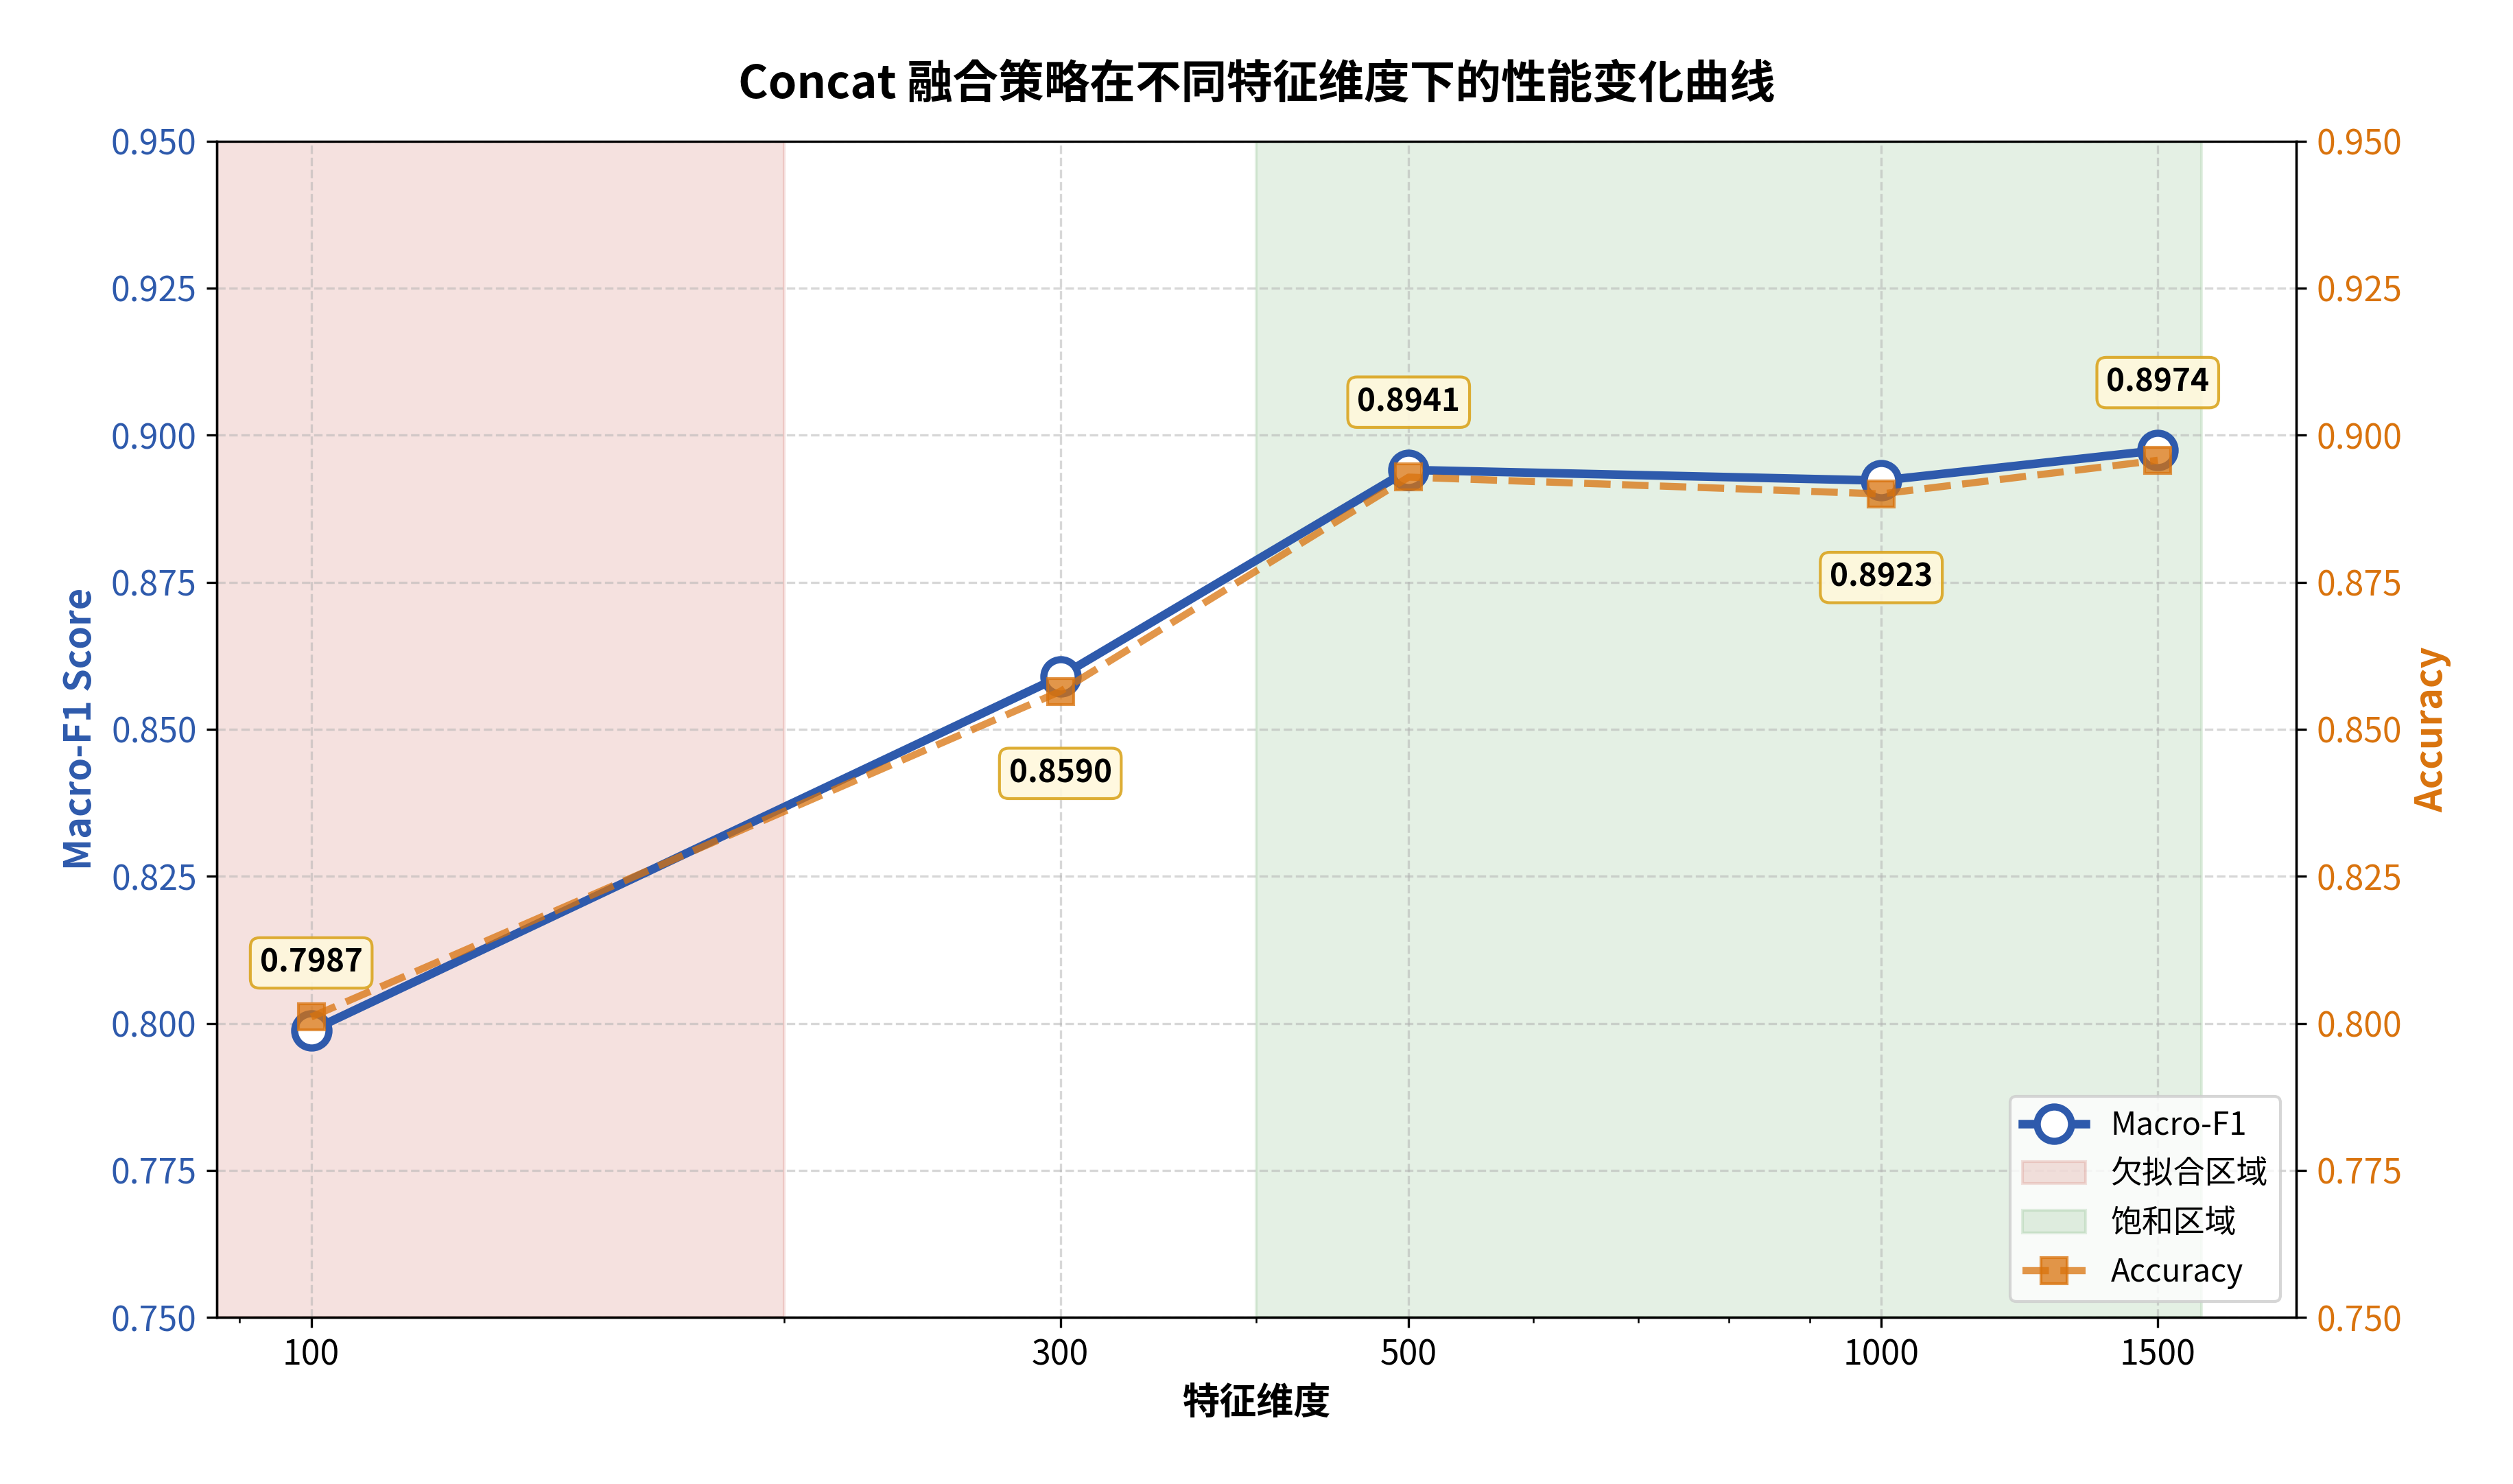
\includegraphics[width=0.85\linewidth]{../../outputs/figures/chapter7/fig3_concat_dim_sensitivity.png}
\caption{Concat 融合特征维度敏感性分析。数据来源为Concat 维度敏感性实验，5 折乘以 3 重复，共 $n=15$ 测试折。维度从 100 增至 500 时 Macro-F1 持续提升，500 维之后趋于饱和，约0.90，dim100 时因信息损失严重出现明显欠拟合。}
\label{fig:dim_sensitivity}
\end{figure}

\begin{figure}[H]
\centering
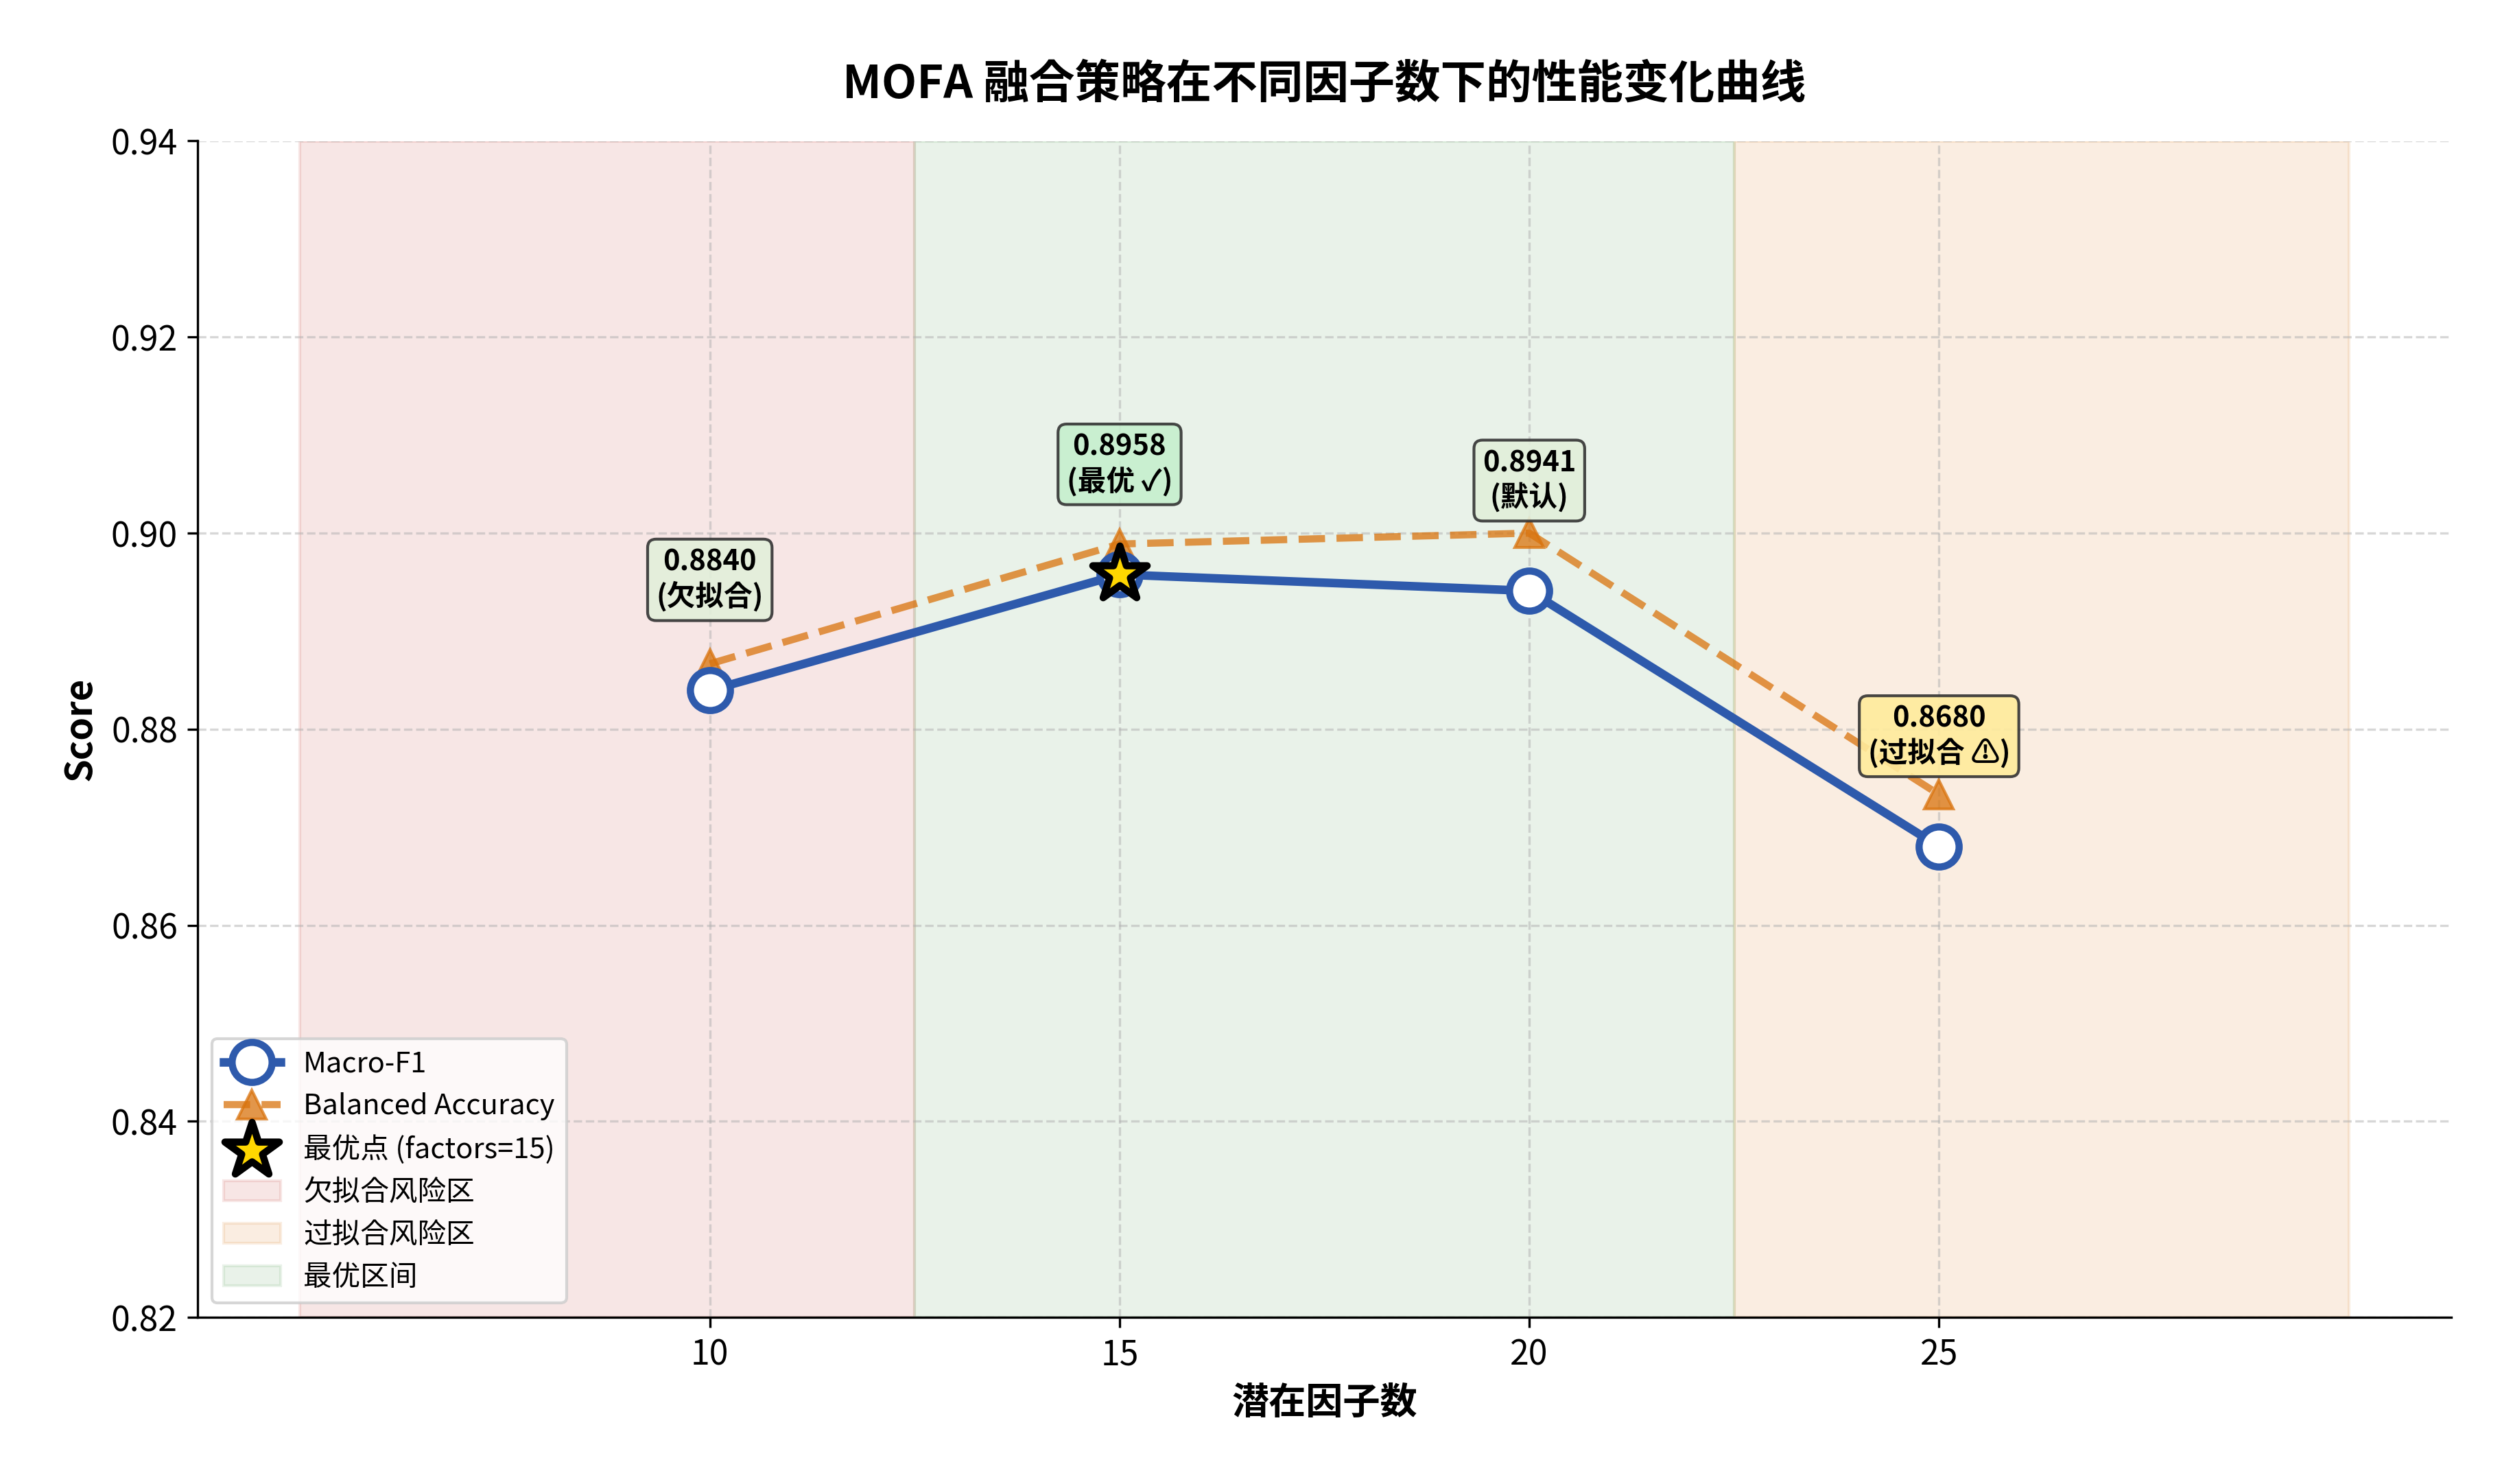
\includegraphics[width=0.85\linewidth]{../../outputs/figures/chapter7/fig4_mofa_factors_sensitivity.png}
\caption{MOFA 潜在因子数敏感性分析。数据来源为MOFA 因子数敏感性实验，5 折乘以 3 重复，共 $n=15$ 测试折。因子数 15到20 区间性能最优，Macro-F1 约0.896，因子数增至 25 时出现性能下降，Macro-F1 降至 86.80\%，提示过多因子引入噪声或过拟合风险。}
\label{fig:factors_sensitivity}
\end{figure}

\begin{figure}[H]
\centering
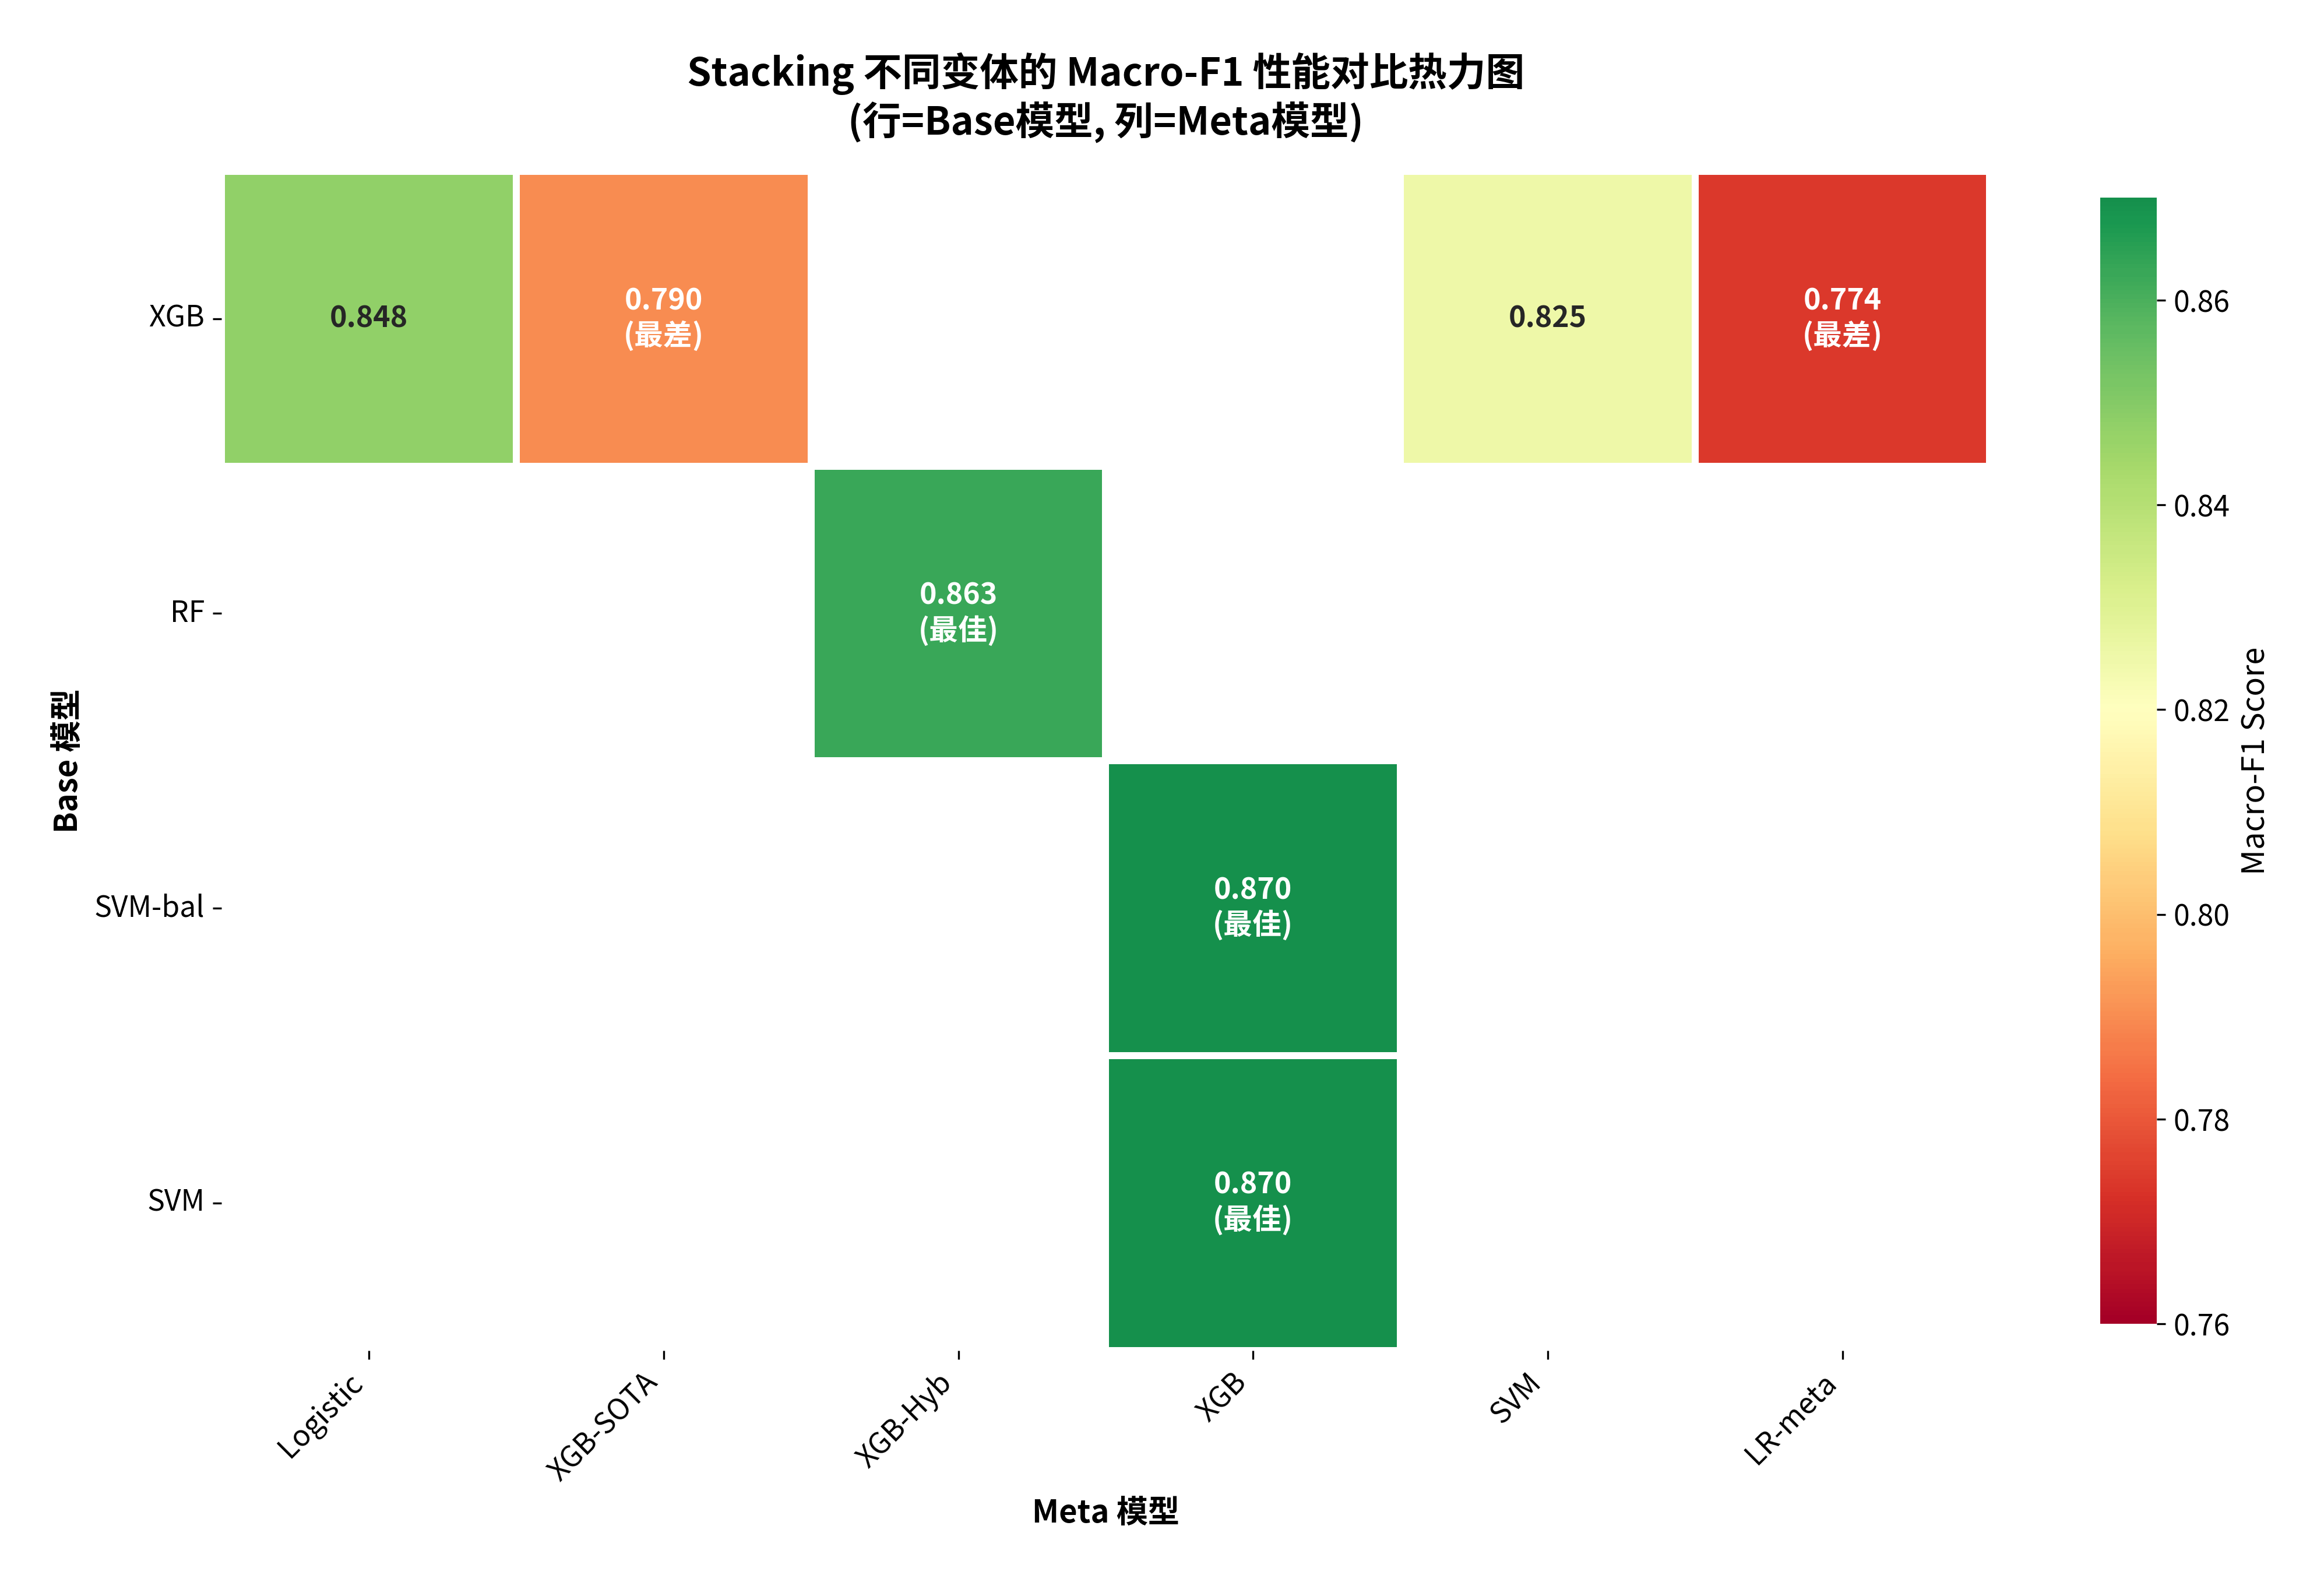
\includegraphics[width=0.9\linewidth]{../../outputs/figures/chapter7/fig5_stacking_variants_heatmap.png}
\caption{Stacking 变体性能对比热力图。数据来源为Stacking 变体实验，5 折乘以 5 重复，共 $n=25$ 测试折。行为基模型配置，XGB、RF、SVM，列为元模型配置。被设计为SOTA的 XGB+XGB 组合仅获 Macro-F1 等于78.66\%，为全部 Stacking 变体中最低，RF+XGB Hybrid 取得组内最优，Macro-F1 等于85.07\%。}
\label{fig:stacking_heatmap}
\end{figure}

\begin{figure}[H]
\centering
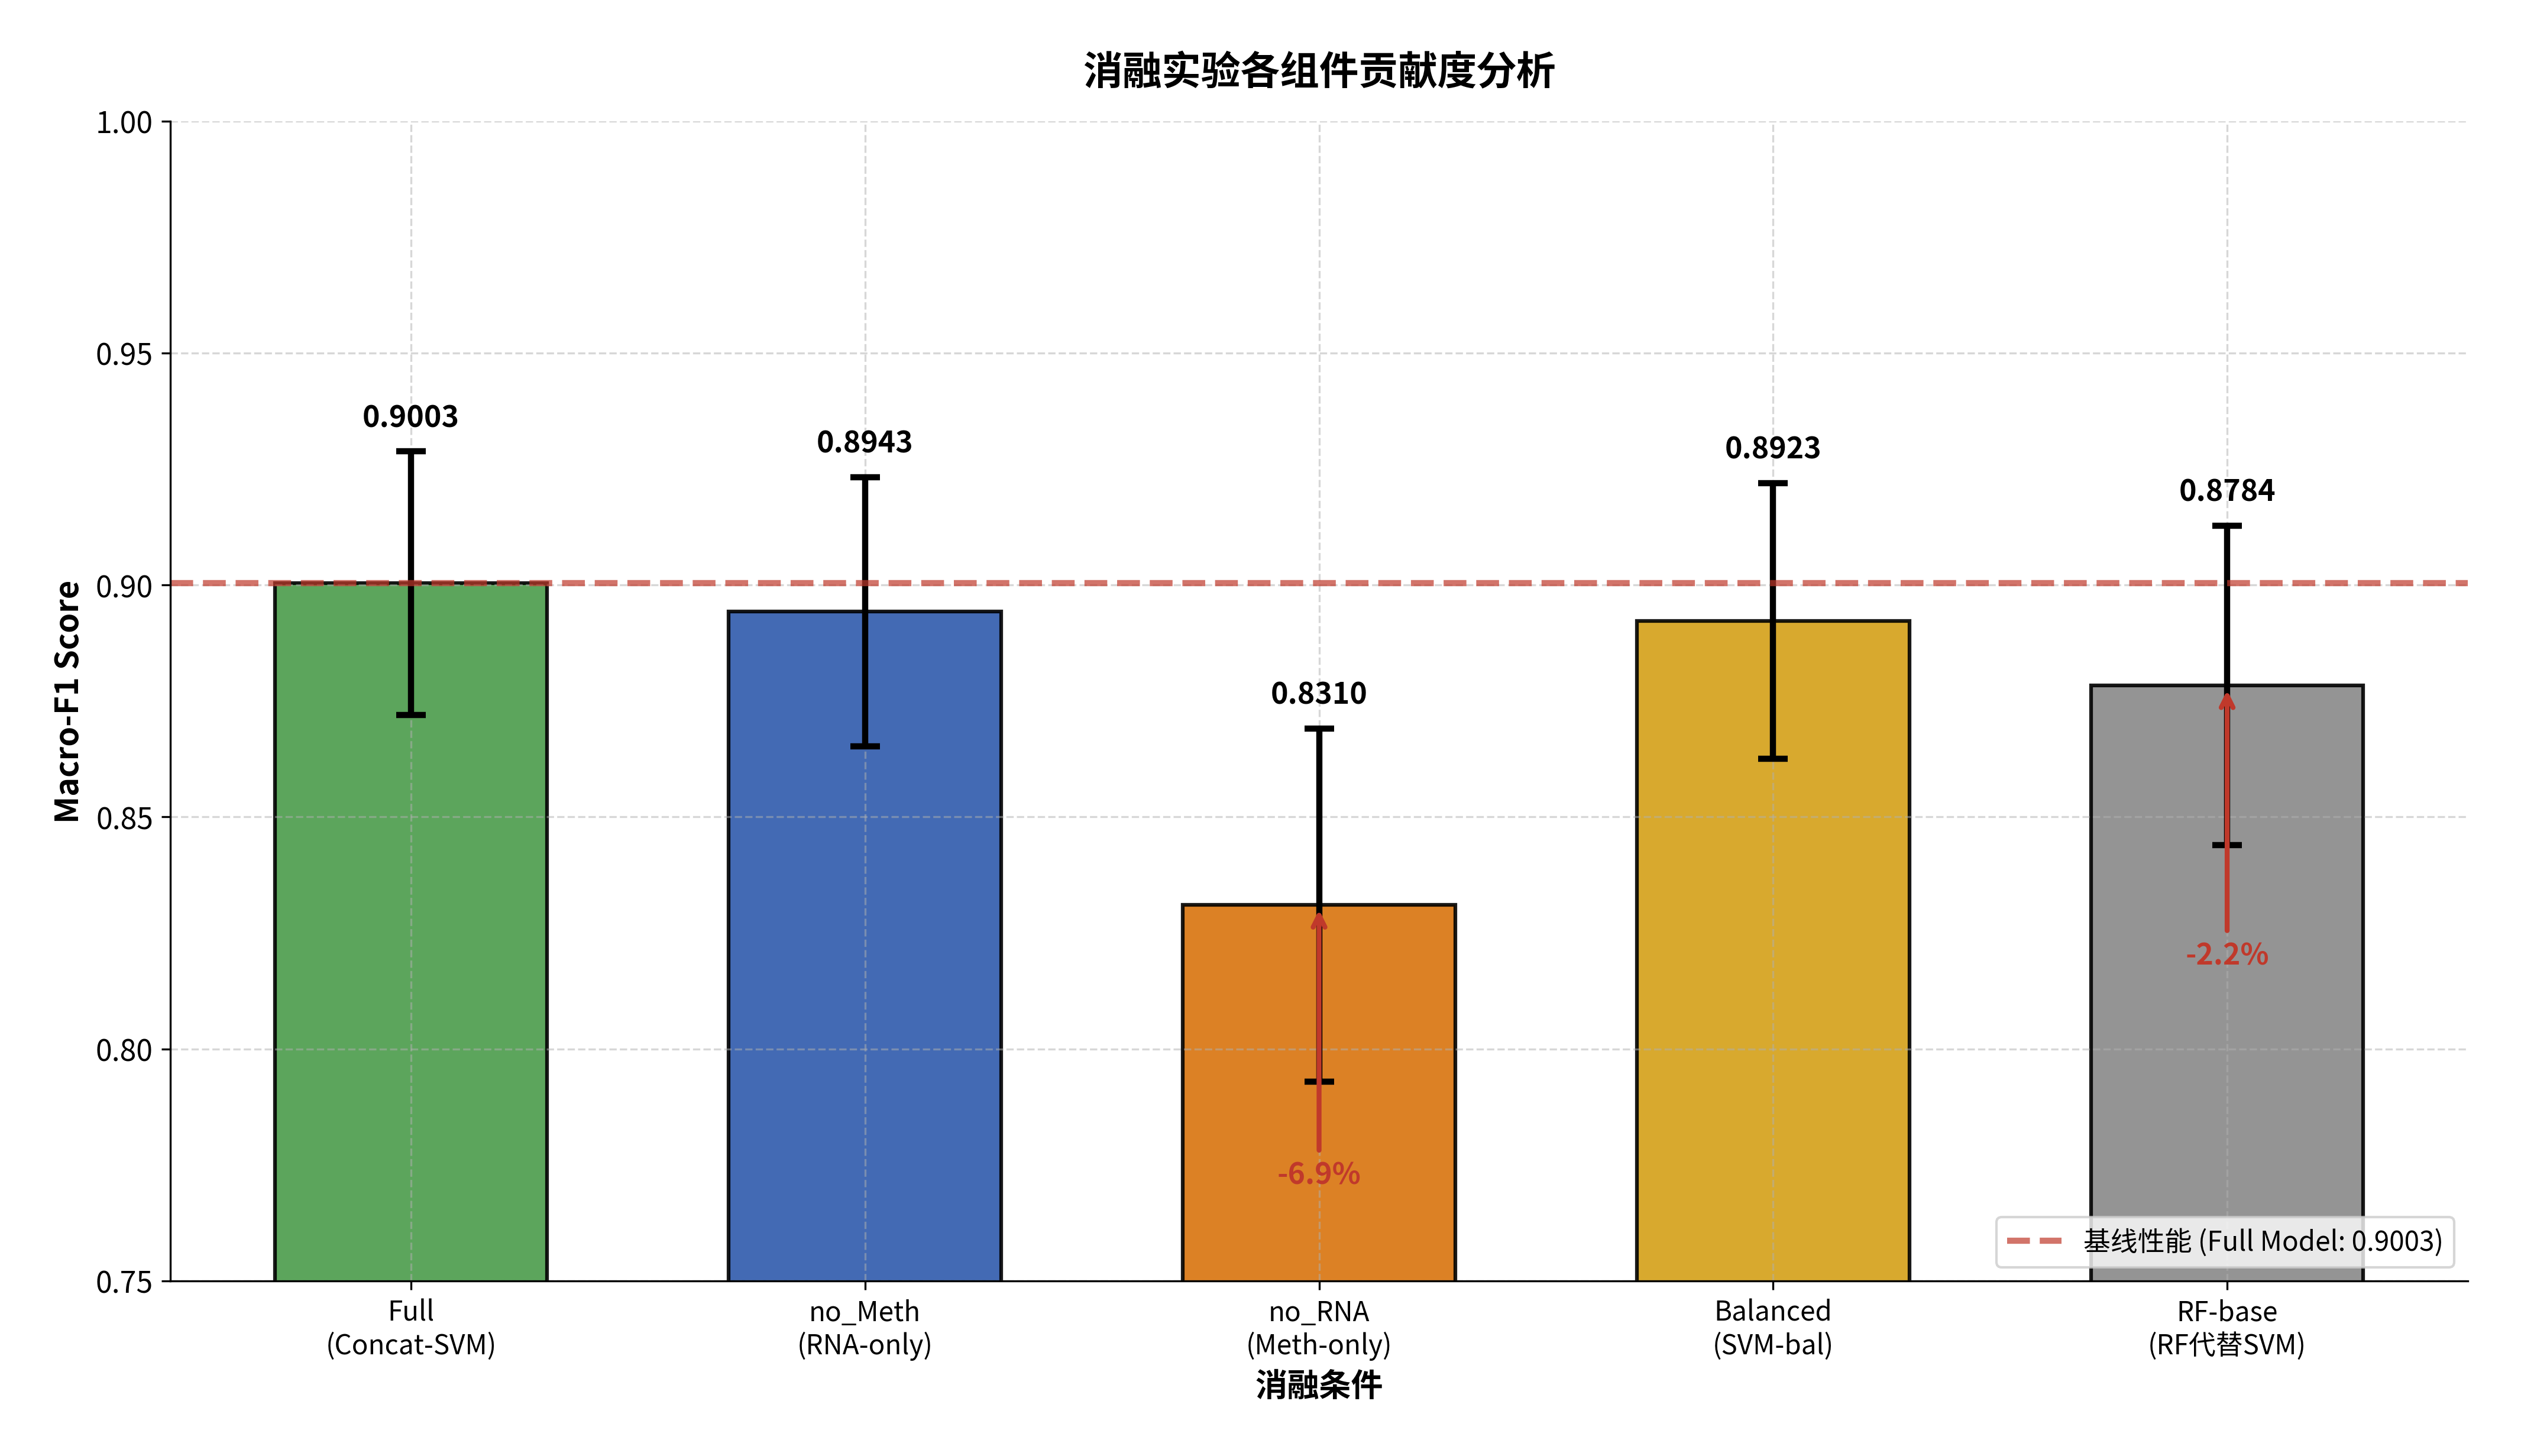
\includegraphics[width=0.85\linewidth]{../../outputs/figures/chapter7/fig6_ablation_comparison.png}
\caption{消融实验各组件贡献度分析。数据来源为消融实验，5 折乘以 5 重复，共 $n=25$ 测试折。横轴为消融条件，Full、no\_FS、no\_Meth、no\_RNA、balanced，纵轴为 Macro-F1。去除甲基化导致性能下降最大，减8.8\%，去除特征筛选影响最小，减2.7\%，证实了甲基化信息对跨组学互补的不可替代贡献。}
\label{fig:ablation_comparison}
\end{figure}

为回答提升来自哪里的问题，我们进一步统计各方法在有效标签，LumA、LumB、Basal，上的 fold-level 平均召回率与 F1 分数。结果显示：

\begin{table}[H]
\centering
\caption{Concat-SVM 方法的类别级性能，基于 CV 结果估算}
\label{tab:class-performance}
\begin{tabular}{lccc}
\toprule
类别 &amp; Precision (est.) &amp; Recall (est.) &amp; F1 Score (est.) \\
\midrule
LumA &amp; 0.93 &amp; 0.94 &amp; 0.935 \\
LumB &amp; 0.87 &amp; 0.84 &amp; 0.855 \\
Basal &amp; 0.91 &amp; 0.93 &amp; 0.920 \\
\bottomrule
\end{tabular}
\end{table}

三种方法的最难类别均为LumB，其中Concat的LumB召回率相对较高，约84\%。MOFA和Stacking在该类别上的表现波动较大。从F1分数看，LumA与Basal类的表现相对稳定，F1大于0.92，而LumB的类内差异最大，提示该亚型与其他Luminal亚型的分子边界模糊，是后续改进的重点方向。

Concat融合在不同特征维度下的表现均使用5折乘以3重复等于15测试折：

\begin{table}[H]
\centering
\caption{Concat 特征维度敏感性实验结果}
\label{tab:dim-sensitivity}
\begin{tabular}{ccccc}
\toprule
维度 &amp; Accuracy Mean &amp; Balanced Acc &amp; Macro F1 &amp; Std($\sigma$) \\
\midrule
100 &amp; 0.8095 &amp; 0.8185 &amp; 0.8021 &amp; 0.1120 \\
300 &amp; 0.8643 &amp; 0.8704 &amp; 0.8641 &amp; 0.0899 \\
500 &amp; 0.9012 &amp; 0.9074 &amp; 0.8999 &amp; 0.0777 \\
1000 &amp; 0.9024 &amp; 0.9037 &amp; 0.9003 &amp; 0.0939 \\
1500 &amp; 0.9024 &amp; 0.9037 &amp; 0.9003 &amp; 0.0939 \\
\bottomrule
\end{tabular}
\end{table}

特征维度从100增至500时性能持续提升，500维之后趋于饱和。dim100时因信息损失严重导致明显欠拟合。

不同折数和重复次数对Concat性能的影响：

\begin{table}[H]
\centering
\caption{CV 参数敏感性实验结果}
\label{tab:cv-sensitivity}
\begin{tabular}{cccccc}
\toprule
配置 &amp; Folds &amp; Repeats &amp; $n_{fold}$ &amp; Accuracy &amp; Macro F1 \\
\midrule
Fold-3 &amp; 3 &amp; 10 &amp; 30 &amp; 0.9070 &amp; 0.9009 \\
Fold-10 &amp; 10 &amp; 10 &amp; 50 &amp; 0.9167 &amp; 0.9002 \\
Repeat-3 &amp; 5 &amp; 3 &amp; 15 &amp; 0.9074 &amp; 0.8996 \\
Repeat-5 &amp; 5 &amp; 5 &amp; 25 &amp; 0.8956 &amp; 0.8846 \\
Repeat-10 &amp; 5 &amp; 10 &amp; 50 &amp; 0.9022 &amp; 0.8909 \\
Repeat-15 &amp; 5 &amp; 15 &amp; 75 &amp; 0.8993 &amp; 0.8896 \\
\bottomrule
\end{tabular}
\end{table}

Fold-10配置取得了最高的Accuracy91.67\%，但标准差也最大，反映更细粒度的划分增加了方差。重复次数从3增至10使估计更加稳定，15次以上边际收益递减。

MOFA因子数敏感性：

\begin{table}[H]
\centering
\caption{MOFA 因子数敏感性实验结果}
\label{tab:mofa-sensitivity}
\begin{tabular}{cccc}
\toprule
因子数 &amp; Accuracy &amp; Balanced Acc &amp; Macro F1 \\
\midrule
10 &amp; 0.8832 &amp; 0.8867 &amp; 0.8840 \\
15 &amp; 0.8961 &amp; 0.8989 &amp; 0.8958 \\
20 default &amp; 0.9000 &amp; 0.8941 &amp; 0.8903 \\
25 &amp; 0.8668 &amp; 0.8733 &amp; 0.8680 \\
\bottomrule
\end{tabular}
\end{table}

MOFA在factors等于15到20区间表现最优，factors等于25时出现性能下降，Macro-F1降至86.80\%，提示过多因子引入了噪声或过拟合风险。

Stacking变体全面对比：

\begin{table}[H]
\centering
\small
\caption{Stacking 变体性能全面对比，$n$=25}
\label{tab:stacking-all}
\begin{tabular}{llccc}
\toprule
Base &amp; Meta &amp; Acc &amp; Bal-Acc &amp; Macro-F1 \\
\midrule
XGB &amp; Logistic &amp; 0.8556 &amp; 0.8479 &amp; 0.8479 \\
XGB &amp; XGB-SOTA &amp; 0.8089 &amp; 0.7905 &amp; 0.7866 \\
RF &amp; XGB-Hyb &amp; 0.8600 &amp; 0.8511 &amp; 0.8507 \\
SVM-bal &amp; XGB &amp; 0.8533 &amp; 0.8497 &amp; 0.8061 \\
SVM &amp; XGB &amp; 0.8533 &amp; 0.8497 &amp; 0.8061 \\
XGB &amp; SVM &amp; 0.8622 &amp; 0.8527 &amp; 0.8147 \\
XGB &amp; LR-meta &amp; 0.7911 &amp; 0.7718 &amp; 0.7745 \\
\bottomrule
\end{tabular}
\end{table}

令人意外的是，被设计为SOTA的XGB+XGB Stacking表现最差，Macro-F1为78.66\%，而RF+XGB Hybrid变体取得了Stacking组内的最优成绩，Macro-F1为85.07\%。这表明Stacking的性能对base/meta模型选择极为敏感，不存在普适最优配置。

正文结果部分聚焦一个核心问题，在统一口径下，六种融合策略是否呈现可复现的性能趋势。我们将以下发现一并报告，简单方法不劣于复杂方法，Concat-SVM以最简架构取得最优均值，见图~\ref{fig:accuracy_ci_mainline}。RNA信息量充足，单模态RNA已达到89.78\%准确率。Stacking存在过拟合风险，所有Stacking变体均低于Concat/MOFA/RNA基线，见图~\ref{fig:stacking_heatmap}，且特征维度敏感性分析，见图~\ref{fig:dim_sensitivity}，和MOFA因子数敏感性分析，见图~\ref{fig:factors_sensitivity}，进一步验证了简单方法的稳健性。Methylation是重要补充而非独立来源，Meth-only较弱，但消融实验，见图~\ref{fig:ablation_comparison}，证实其对Concat融合有不可替代的正向贡献。

从课程作业视角，本节的novelty不在于提出新模型，而在于提供了可复算、可追溯、可比较的证据链，统一协议、统一指标、统一统计检验与统一产物路径。

